\documentclass[11pt,a4paper]{article}
\usepackage[utf8]{inputenc}
\usepackage[T1]{fontenc}
\usepackage{geometry}
\usepackage{graphicx}
\usepackage{xcolor}
\usepackage{tikz}
\usetikzlibrary{shapes.geometric, arrows.meta, positioning, fit, backgrounds}
\usepackage{booktabs}
\usepackage{multirow}
\usepackage{hyperref}
\usepackage{fontawesome5}
\usepackage{tcolorbox}
\usepackage{titlesec}
\usepackage{enumitem}

\geometry{margin=1in}
\definecolor{ttured}{RGB}{204,0,0}
\definecolor{accent}{RGB}{0,82,155}
\definecolor{success}{RGB}{34,139,34}
\definecolor{warn}{RGB}{218,165,32}

\hypersetup{
  colorlinks=true,
  linkcolor=accent,
  urlcolor=accent,
  citecolor=accent
}

\titleformat{\section}{\large\bfseries\color{accent}}{\thesection}{1em}{}
\titleformat{\subsection}{\normalsize\bfseries}{\thesubsection}{1em}{}

\begin{document}

% --- Title Block ---
\begin{center}
  {\Large\bfseries CS5374 Project Proposal}\\[0.5em]
  {\normalsize Software Verification and Validation --- Spring 2026}\\[0.3em]
  \colorbox{ttured!15}{\parbox{0.9\textwidth}{\centering\bfseries\color{ttured}
    Trustworthy AI Legal and Governmental Content Validator\\
    \small Verification of Legal News Sources, Officials, Laws, Court Documents, and Templates
  }}\\[1em]
  \faIcon{users} \textit{Scope: Trustworthy AI}
\end{center}
\vspace{0.5em}

% --- Introduction ---
\section*{\faIcon{info-circle} Introduction}

Large language models and retrieval-augmented generation (RAG) systems have become powerful tools for answering questions about legal and governmental matters, yet they frequently hallucinate or return outdated information. When these systems invent judge names, cite non-existent laws, fabricate election details, or surface unverified court documents, the consequences can be serious: litigants may receive incorrect legal advice, public officials may be misrepresented, and invalid ordinances or statutes may be cited as binding authority. This project addresses that risk by building a Trustworthy AI validation pipeline that verifies legal and governmental content against authoritative sources before any AI system presents it to users. The overarching purpose is to ensure that information about legal news, judges, elected officials, elections, laws, court documents, and legal templates is grounded in verifiable data and that every output includes clear provenance.

% --- Summary ---
\section*{\faIcon{file-alt} Summary}

The proposed system will use LangChain and LangGraph to construct validator agents that ingest, parse, and verify structured content at each stage of the pipeline. For legal news sources, the system will check URLs against domain trust lists and integrate with fact-check and media bias services such as NewsGuard and AllSides. Judge names will be validated against federal and state court rosters maintained by the U.S. Courts and state judicial directories. Elected officials and their terms will be verified using official government APIs and Secretary of State election board data, supplemented by curated sources such as Ballotpedia where source provenance is explicitly checked. Election details and opponents will be grounded in certified filings and results from state election boards and the Federal Election Commission. City, county, and state laws and ordinances will be verified against municipal code repositories such as eCode360 and state legislature databases. Court documents, including filings, opinions, and dockets, will be validated through PACER, the CourtListener API, and state court e-filing systems. Legal document templates will be checked against official court form registries and verified via checksum validation. The pipeline will enforce schema validation and source grounding at every stage, and only content that passes verification will be indexed and made available to downstream AI systems. All outputs will carry provenance metadata indicating the source, date, and verification status, so that users and systems can assess the trustworthiness of the information they receive.

% --- Personnel ---
\section*{\faIcon{user-friends} Project Personnel}
\begin{tcolorbox}[colback=gray!5, colframe=accent!50, title=\faIcon{pencil-alt} Add team member names and TTU emails]
  \begin{itemize}[noitemsep]
    \item \underline{\hspace{6cm}}
    \item \underline{\hspace{6cm}}
    \item \underline{\hspace{6cm}}
  \end{itemize}
\end{tcolorbox}

% --- Executive Summary ---
\section*{\faIcon{lightbulb} Executive Summary}

\begin{itemize}[leftmargin=*]
  \item[\faIcon{exclamation-triangle}] \textbf{Problem:} LLMs and RAG systems frequently hallucinate or return outdated legal and governmental information, including fake judge names, non-existent laws, fabricated election details, and unverified court documents. Errors in this domain cause serious harm (misadvising litigants, misrepresenting officials, citing invalid laws).
  
  \item[\faIcon{project-diagram}] \textbf{Approach:} Build a Trustworthy AI validation pipeline that ingests, indexes, and verifies structured content against authoritative sources before any AI system surfaces it to users.
  
  \item[\faIcon{list-check}] \textbf{Content types:} Legal news sources (with bias/fact-check ratings), judge names (federal/state benches), elected official names and terms, election details and opponents, city/county/state laws and ordinances, court documents (filings, opinions, dockets), and legal document templates.
  
  \item[\faIcon{cogs}] \textbf{Method:} Use \href{https://langchain.com}{LangChain}/\href{https://langchain-ai.github.io/langgraph}{LangGraph} to construct validator agents; integrate APIs and scrapers for official registries (e.g., state courts, election boards, municipal codes); enforce schema validation and source grounding at each pipeline stage.
  
  \item[\faIcon{shield-alt}] \textbf{Trust signal:} Only content that passes verification against authoritative databases is returned; all outputs include provenance (source, date, verification status).
\end{itemize}

% --- Pipeline Diagram ---
\section*{\faIcon{sitemap} Validation Pipeline Architecture}

\begin{center}
\begin{tikzpicture}[
  node distance=0.8cm and 1.2cm,
  box/.style={rectangle, draw=accent!70, fill=accent!5, rounded corners, minimum width=2.2cm, minimum height=0.6cm, font=\small},
  validator/.style={diamond, draw=success!70, fill=success!10, aspect=2.5, font=\small},
  arrow/.style={-{Stealth[length=2mm]}, thick, accent!70}
]
  \node[box] (ingest) {\faIcon{download} Ingest};
  \node[box, right=of ingest] (parse) {\faIcon{code} Parse};
  \node[validator, right=of parse] (valid) {\faIcon{check} Verify};
  \node[box, above right=0.6cm and 1cm of valid] (pass) {\faIcon{check-circle} Pass};
  \node[box, below right=0.6cm and 1cm of valid] (fail) {\faIcon{times-circle} Fail};
  \node[box, right=2.5cm of pass] (output) {\faIcon{database} Index};
  
  \draw[arrow] (ingest) -- (parse);
  \draw[arrow] (parse) -- (valid);
  \draw[arrow] (valid) -- node[above, font=\tiny] {verified} (pass);
  \draw[arrow] (valid) -- node[below, font=\tiny] {reject} (fail);
  \draw[arrow] (pass) -- (output);
\end{tikzpicture}
\end{center}

% --- Deliverables ---
\section*{\faIcon{rocket} Deliverables}

\subsection*{\faIcon{flag-checkered} First Round}
\begin{enumerate}[leftmargin=*]
  \item Design document and threat model for the validation pipeline (prompt injection, data poisoning, source spoofing).
  \item Implemented validator modules for: (1) legal news source verification (URL, domain trust, fact-check API); (2) judge name verification against federal/state court rosters; (3) elected official verification against official government APIs or scraped registries.
  \item LangGraph prototype with validator nodes that route outputs to pass/fail based on verification checks.
  \item Unit tests and integration tests for each validator; documented test coverage for Trustworthy AI criteria.
\end{enumerate}

\subsection*{\faIcon{trophy} Final / Second Round}
\begin{enumerate}[leftmargin=*]
  \item Full validator suite: legal news, judges, elected officials, election details and opponents, city/county/state laws, court documents, and templates.
  \item Integration with at least one authoritative source per content type.
  \item End-to-end RAG pipeline with validation gates; only verified content is retrievable.
  \item Security review report (red-team results for prompt injection, data exfiltration, tool abuse).
  \item 15--20 minute presentation demonstrating the validator pipeline, trust guarantees, and lessons learned.
\end{enumerate}

% --- Appendix Table with Links ---
\section*{\faIcon{table} Appendix: Content Types and Verification Strategies}

\begin{table}[h]
\centering
\small
\begin{tabular}{@{}lll@{}}
\toprule
\textbf{Content Type} & \textbf{Verification Strategy} & \textbf{Example Sources} \\
\midrule
\faIcon{newspaper} Legal news & Domain trust, fact-check APIs & \href{https://www.newsguardtech.com}{NewsGuard}, \href{https://www.allsides.com}{AllSides} \\
\faIcon{gavel} Judge names & Federal/state court rosters & \href{https://www.uscourts.gov}{U.S. Courts}, state courts \\
\faIcon{landmark} Elected officials & Gov APIs, election boards & State SOS, \href{https://ballotpedia.org}{Ballotpedia} \\
\faIcon{vote-yea} Election details & Certified filings, results & State boards, \href{https://www.fec.gov}{FEC} \\
\faIcon{balance-scale} Laws & Code repositories, statutes & \href{https://www.ecode360.com}{eCode360}, legislatures \\
\faIcon{file-alt} Court documents & PACER, CourtListener & \href{https://www.pacer.gov}{PACER}, \href{https://www.courtlistener.com}{CourtListener} \\
\faIcon{file-signature} Templates & Verified form registry & Official court forms \\
\bottomrule
\end{tabular}
\caption{Content types with verification strategies and authoritative source links.}
\end{table}

% --- Threat Model Diagram ---
\section*{\faIcon{bug} Threat Model}

\begin{center}
\begin{tikzpicture}[
  node distance=0.6cm,
  asset/.style={rectangle, draw=accent, fill=accent!10, rounded corners, minimum width=1.8cm, font=\small},
  threat/.style={rectangle, draw=warn, fill=warn!15, rounded corners, minimum width=1.6cm, font=\small},
  arrow/.style={->, thick, red!70}
]
  \node[asset] (user) {\faIcon{user} User Data};
  \node[asset, right=1.5cm of user] (kb) {\faIcon{database} Internal KB};
  \node[asset, right=1.5cm of kb] (tools) {\faIcon{tools} Tool Access};
  
  \node[threat, below=1.2cm of user] (inj) {\faIcon{exclamation} Prompt Injection};
  \node[threat, below=1.2cm of kb] (poison) {\faIcon{flask} Data Poisoning};
  \node[threat, below=1.2cm of tools] (extract) {\faIcon{copy} Model Extraction};
  
  \draw[arrow] (inj) -- (user);
  \draw[arrow] (inj) -- (tools);
  \draw[arrow] (poison) -- (kb);
  \draw[arrow] (extract) -- (kb);
\end{tikzpicture}
\end{center}

% --- Media Links Box ---
\section*{\faIcon{link} Key Media \& Resource Links}

\begin{tcolorbox}[colback=accent!5, colframe=accent]
  \textbf{Frameworks \& Tools:}\\
  \faIcon{link} \href{https://langchain.com}{LangChain} \quad
  \faIcon{link} \href{https://langchain-ai.github.io/langgraph}{LangGraph} \quad
  \faIcon{link} \href{https://smith.langchain.com}{LangSmith} \quad
  \faIcon{link} \href{https://github.com/NVIDIA/garak}{GARAK (red-teaming)}\\[0.5em]
  \textbf{Data \& Verification:}\\
  \faIcon{link} \href{https://www.newsguardtech.com}{NewsGuard} \quad
  \faIcon{link} \href{https://www.courtlistener.com/api}{CourtListener API} \quad
  \faIcon{link} \href{https://www.pacer.gov}{PACER} \quad
  \faIcon{link} \href{https://www.fec.gov}{FEC}
\end{tcolorbox}

\vspace{1em}
\begin{center}
  \faIcon{copyright} CS5374 Spring 2026 --- Trustworthy AI
\end{center}

\end{document}
